\item[(a)]

\begin{itemize}
\item[1.]
Define $\mathbf{w}= (-1,-1)$, $\theta = 0$ 
\item[2.]
$\mathbf{w} = (-\frac{1}{2},-\frac{1}{2})$, $\theta = 0$ 
\item[3.]
We are finding a line that the distance from the point to the line represents the absolute value of $\vec{w}^T\vec{x}$ and the different side of the line represents the sign of $\vec{w}^T\vec{x}$. To maximize the margin, I consider the perpendicular bisectors of the closest pair of positive point and negative point, (-2,0) and (0,2). If I find the perpendicular bisector with distance to the points which is also the minimal distance of all points to this line, the line is the separator we are looking for.
\\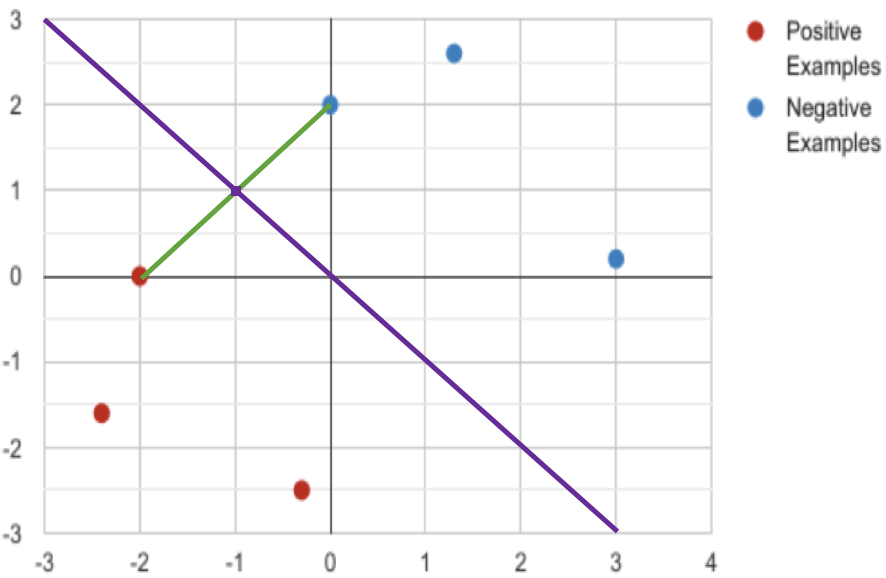
\includegraphics[width = 0.7\textwidth]{fig2.png}\\
\end{itemize}
\item[(b)]
\begin{itemize}
\item[1.]
As mentioned above, the support vectors are point 1 and point 6 which means I = \{1,6\}.
\item[2.]
 $\mathbf{w}^{*} = \sum \alpha_i y_i x_i \Rightarrow (-\frac{1}{2},-\frac{1}{2}) =\alpha_1\times 1 \times(-2,0)+\alpha_2\times -1\times(0,2) $.\\ Thus, $\{\alpha_1, \alpha_2\}=\{0.25,0.25\}$.  
\item[3.]
Objective function: $\frac{1}{2}||w||^2$ ($||w||$ calculated by L2 norm).\\
Objective function value $=\frac{1}{2}||w||^2 = \frac{1}{2} [(-0.5)^2+(-0.5)^2)] = 0.25 $.
\end{itemize} 
\item[(c)]
\textbf{For the case $C = 0$}, it shows that the algorithm will find the $w$ with the minimal absolute value without considering the loss. Thus, $\xi_i$ can be really big that the result can not separate the dataset anymore. More specifically, the algorithm will get $\bb{w} = \bb{0}$ and $\xi_{i} \ge 1$ which minimizing the objective function being zero, but representing nothing for separating the points. Thus, the smaller C we assign the better generalization we make, but C = 0 is too general that any dataset will satisfy the answer. \\
\textbf{For the case $C = \infty$}, the algorithm will try to make the term $\sum_{j=1}^{m}{\xi_{i}}$ zero because if there is anything nonzero in that term, the objective function value will blow up to $\infty$. Thus, all $\xi_{i}$ should be zero, and that makes the algorithm find $w$ with the most strict margin as \textbf{Hard SVM}. \textbf{The result would be the same as I have found in (a)-2.}\\
\textbf{For the case $C = 1$}, it is a balanced option between $C = 0$ and $C = \infty$. The algorithm will get us a $w$ between $w$ with the most strict margin and $w$ allowing any amount of loss. Thus, we will get a general and good solution for the dataset.

  